% !TEX encoding = UTF-8
% !TEX TS-program = pdflatex
% !TEX root = ../tesi.tex
% !TEX spellcheck = it-IT

%**************************************************************
\chapter{Realtà aziendale}
\label{cap:realta}
%**************************************************************

\intro{Questo capitolo serve per descrivere l'azienda e il dominio applicativo
in cui ha trovato collocazione lo stage.}

%**************************************************************
\section{L'azienda}

Sanmarco Informatica è una software house avente sede a Grisignano di Zocco
(Vicenza) e filiali a Udine, Reggio Emilia, Milano e Roma.

Operante da più di 20 anni nel campo degli applicativi di tipo gestionale con
più di 210 collaboratori, Sanmarco Informatica è all'interno di un pool di
aziende chiamato Pool Galileo, il cui scopo è promuovere l'\gloss{erp}
Jgalileo in tutta Italia.

Grazie ad una politica commerciale condivisa tra queste aziende, i suoi
prodotti vengono diffusi su tutto il territorio nazionale a clienti di diversa
dimensione e diverso settore merceologico.

L'azienda prende decisioni principalmente in base ai bisogni dei clienti,
identificando in questi la buona riuscita dei suoi progetti. È proprio per
questo motivo che le soluzioni che Sanmarco Informatica propone sono spesso
personalizzate in base alle necessità specifiche di ciascun cliente.

Tale aspetto della filosofia aziendale si può notare anche da come essa stessa
è riuscita a mutare nel corso degli anni, rimanendo sensibile alle variazioni
del mercato ed adattando i propri prodotti e processi in funzione di queste.

\begin{figure}[H]%
\centering

\includegraphics[width=.5\columnwidth]{immagini/logo-sanmarco.jpg}
\caption{Logo di Sanmarco Informatica}%
\label{fig:logo-smi}%
\end{figure}

%**************************************************************
\section{Prodotti e servizi offerti}

L'azienda offre molti servizi ai propri clienti:

\begin{itemize}
	\item Analisi e progettazione della soluzione per il cliente, per mezzo di un
	dialogo diretto che riesca a identificare i bisogni necessari per un prodotto
	che soddisfi pienamente le attese;
	\item Installazione ed avviamento delle soluzioni, una volta sviluppate;
	\item Formazione per l'uso delle proprie applicazioni, che può essere
	effettuata sia in sede propria che dal cliente;
	\item Consulenza, sia in ambito informatico che economico-gestionale;
	\item Assistenza, che può essere di tipo sistemistico, \gloss{helpdesk} o
	applicativo. Questo ultimo tipo di assistenza può essere effettuato a distanza
	con software come \gloss{teamviewer} o con interventi sul posto.
\end{itemize}

Sanmarco Informatica offre diversi prodotti a privati: di seguito verranno
descritti solamente JPA (l'applicazione estesa durante l'attività di stage) e
Jgalileo (l'applicazione su cui vengono concentrate principalmente le risorse
aziendali).

Tuttavia è doveroso far notare che questi non sono gli unici prodotti offerti
dall'azienda: sono presenti numerose applicazioni verticali per alcuni clienti
e altri progetti, come ad esempio 4words.

\subsection{JPA}

Il \gloss{bpm} definisce un insieme di teorie manageriali atte ad allineare i
processi aziendali con le esigenze dei clienti. Con questa nuova visione, le
principali risorse aziendali non sono più le funzioni all'interno di
un'azienda, ma i suoi processi. Tali teorie acquistano concretezza grazie ad
una web application offerta da Sanmarco Informatica, JPA (\emph{Java Process
Architect}), che permette la modellazione di processi e l'analisi della loro
evoluzione nel tempo.

JPA si pone come obiettivo di fornire all'utente un'interfaccia comprensibile e
facilmente utilizzabile. In questo modo, anche un utente privo di specifiche
abilità informatiche riesce ad utilizzare l'applicazione senza particolari
sforzi.

L'architettura ad alto livello dell'applicazione è il modello client-server.
Infatti, per rispondere alle richieste che pervengono dal lato client (o
\FREND{}), il \BKEND{} esegue:

\begin{itemize}
	\item le operazioni \gloss{crud} sul database JPADb, al quale il \FREND{} non
	ha direttamente accesso;
	\item le elaborazioni di dati che hanno carico computazionale elevato.
\end{itemize}

Il \FREND{} a sua volta fornisce un'interfaccia utente \emph{user-friendly}
visualizzabile tramite un browser da cui l'utente può interagire con JPA.

JPA si compone di diverse aree, che identificano un insieme di moduli
raggruppati in base alla finalità a cui sono indirizzati.

Tali aree sono:

\begin{itemize}
	\item \textbf{Processi}, in cui vengono gestiti processi e relativi cardini
	(termine utilizzato equivalentemente a \gloss{milestone});
	\item \textbf{Ricerca}, in cui si possono ricercare informazioni sui
	processi;
	\item \textbf{Configurazione}, in cui l'amministratore di sistema può
	impostare le proprie preferenze generiche di utilizzo;
	\item \textbf{Audit}, dove è possibile vedere resoconti su dati presenti in
	JPA;
	\item \textbf{Scrum}, attualmente utilizzata per la gestione solamente
	interna dei processi;
	\item \textbf{Forum}, utilizzata come spazio di discussione, punto di
	raccolta di informazioni comuni e luogo di condivisione di conoscenze;
	\item \textbf{Calendario}, in cui vi è una classica visuale mensile di
	calendario ed ogni casella presente riporta gli impegni o le scadenze per
	quel giorno;
	\item \textbf{Mail}, utilizzata per lo scambio di messaggi di posta
	elettronica interna a JPA;
	\item \textbf{Utente}, in cui l'utente può vedere le proprie informazioni ed
	eventualmente modificarne alcune.
\end{itemize}

L'accesso alle aree sopra elencate è permesso solamente se l'utente possiede
una qualifica adeguata: nell'utilizzo come utente-membro del team ho
avuto accesso solamente alle ultime cinque aree, mentre durante lo sviluppo
delle nuove funzionalità ho avuto pieno accesso a tutte le aree di JPA,
effettuando l'accesso come amministratore.

L'area Scrum di JPA, come detto prima, è dedicata alla gestione interna dei
processi del team in cui sono stato inserito. Questa parte dell'applicazione
fornisce strumenti a supporto della metodologia Scrum adottata dal team,
alleggerendo l'attività di pianificazione.

\begin{figure}[H]%
\centering
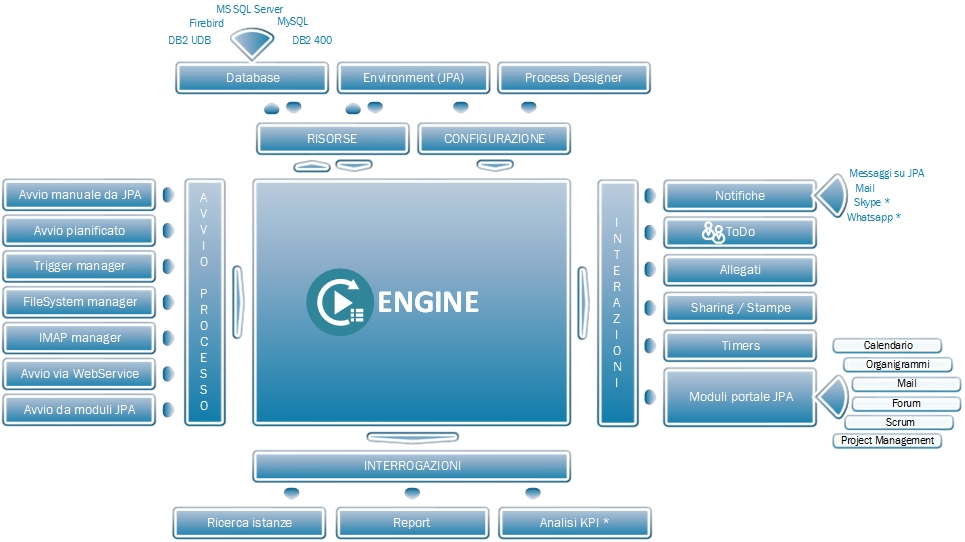
\includegraphics[width=.8\columnwidth]{immagini/jpa-strutt}%
\caption{Struttura di JPA}%
\label{fig:strutt-jpa}%
\end{figure}
%--------------------------------------------------------------
\subsection{Jgalileo}
Jgalileo è una \gloss{suite} di pacchetti software che messi insieme compongono
un applicativo di tipo gestionale che è in grado di supportare i vari processi
di un'azienda.

Questo \gloss{erp}, prodotto di punta di Sanmarco Informatica, è usato
quotidianamente da più di 1500 aziende, per un totale di oltre 50000 utenti.
Queste aziende operano in diversi mercati: alimentare, commerciale, serramenti,
cantine e distillerie sono solo alcuni di questi.

A seconda delle estensioni (chiamate \textbf{moduli}) richieste dal cliente,
il prodotto può essere specializzato per diverse aree. Alcune di queste sono
amministrazione e finanza, CRM, controllo di gestione, archiviazione
documentale, commerciale, produzione, rilevazione dati, gestione processi,
qualità e business intelligence.

%**************************************************************
\section{Scrum aziendale}

Sanmarco Informatica ha mantenuto fedeltà alla propria \gloss{mission} anche
per quanto riguarda l'organizzazione dei propri processi aziendali.

Al fine di restare attenta alle possibili variazioni delle esigenze dei
clienti, dal 2013 l'azienda ha deciso di abbracciare i principi espressi
nell'\gloss{agilemanifesto}, organizzando i propri team con la metodologia
Scrum.

\subsection{Metodologia Scrum}

Questo approccio è ritenuto un \gloss{framework} dai suoi stessi creatori,
poichè permette di avere notevoli benefici al costo di seguire le sue regole e
le sue linee guida.

La metodologia Scrum infatti rivoluziona l'approccio classico di sviluppo
software a partire dalle sue unità più piccole: i team di sviluppo (in Scrum,
\emph{Development Team}).

Nei progetti ad impostazione ``classica'', un team di sviluppo può avere
composizione variabile a seconda delle persone che ne vengono inserite e
rimosse: tra queste, i ruoli più comuni su cui si basa l'alternanza dei membri
di un gruppo sono analisti, progettisti e programmatori.

In Scrum, la composizione di un team è fissa, poichè un team non cambia
\textbf{mai} i propri componenti se non per cause indipendenti dallo sviluppo
del prodotto su cui il team sta lavorando. Ciò è possibile perchè i
\emph{Development Team} in Scrum sono:

\begin{itemize}
	\item \emph{self-organizing}, ovvero si ripartiscono da soli il lavoro senza
	che un Responsabile di Progetto (o un membro avente funzioni equivalenti a
	questo) assegni loro le attività;
	\item \emph{cross-functional}, in quanto un \emph{Development Team} è nel suo
	complesso competente in tutto ciò di cui necessita per portare a termine un
	progetto.
\end{itemize}

Per quanto si vede nei due punti sovrastanti, è facile notare che i ruoli
classici di progetto scompaiono, o quantomeno vengono gestiti internamente e
flessibilmente all'interno di un team di sviluppo Scrum (termine inglese
utilizzato nel rugby che significa \textbf{mischia ordinata}).

\begin{figure}%
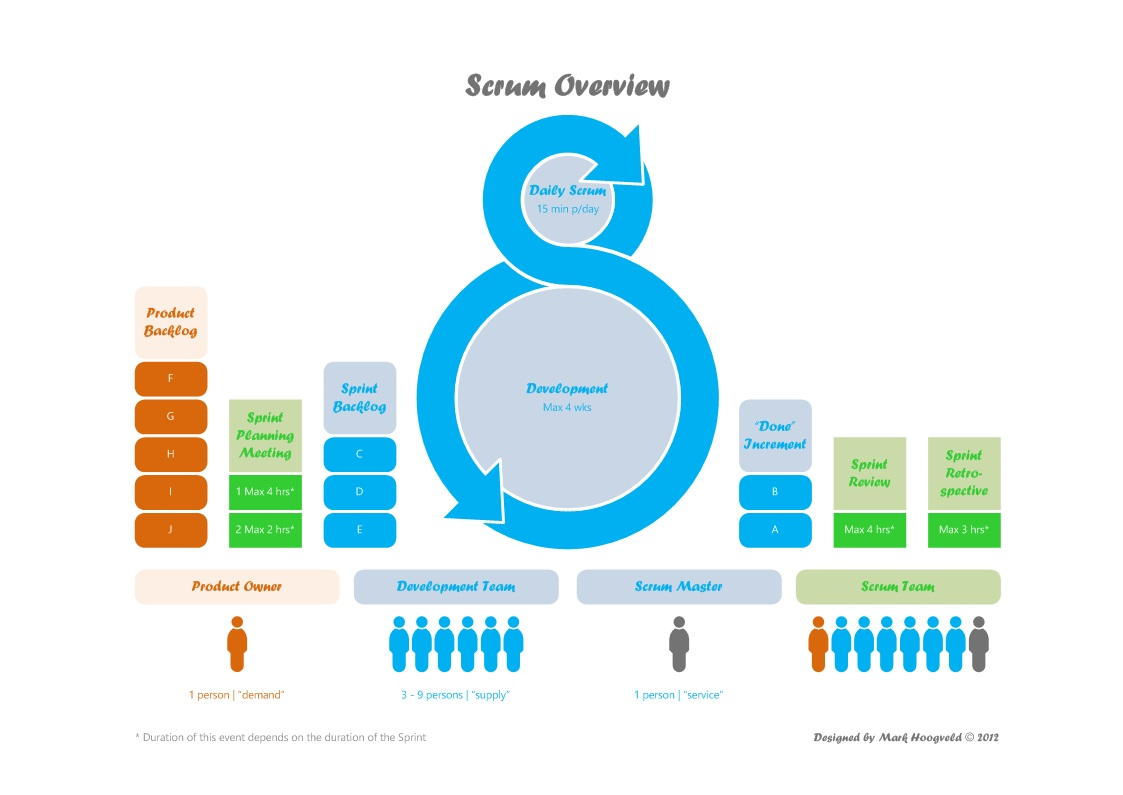
\includegraphics[width=\columnwidth]{immagini/scrum-schema}%
\caption{Flusso di sviluppo software in Scrum}%
\label{fig:scrum-schema}%
\end{figure}

Un'altra differenza rispetto all'approccio classico dello sviluppo software si
ha nelle misure del team di sviluppo. In Scrum i gruppi hanno dimensione
massima di nove persone, sebbene la dimensione consigliata dagli ideatori sia
di sette membri. Limitando il numero di persone che devono lavorare insieme, la
difficoltà organizzativa viene notevolmente ridotta e il gruppo può
concentrarsi maggiormente sullo sviluppo del prodotto e aver meno problemi
dovuti alla coordinazione interna.

Questo beneficio è ottenibile grazie anche ai due ulteriori ruoli che Scrum
prevede: lo \emph{Scrum Master} ed il \emph{Product Owner}.

Lo \emph{Scrum Master} è la guida dell'intero \emph{Scrum Team} affinchè la
metodologia sia applicata correttamente. Il suo ruolo ha importanza
fondamentale poichè, come riconoscono gli stessi ideatori, Scrum può portare a
conseguenze molto negative se applicato scorrettamente.

Lo \emph{Scrum Master} valuta la qualità dei processi, li ispeziona e fornisce
al resto del gruppo soluzioni per diminuire gli sprechi di risorse e
massimizzare il valore delle interazioni tra i componenti del gruppo.

Il \emph{Product Owner} consente invece al \emph{Development Team} di
continuare lo sviluppo del prodotto senza continue interruzioni dovute
al dialogo con i portatori di interesse (\emph{stakeholders}) esterni allo
\emph{Scrum Team} o alla continua variazione dei requisiti.

Egli è responsabile del carico di lavoro (chiamato \emph{backlog}) presente per
il \emph{Development Team} e si interfaccia costantemente con quest'ultimo per
determinare la priorità e stimare lo sforzo necessario per portare a termine
ciascun task, ovvero un'attività il cui completamento comporta il
soddisfacimento di un requisito utente.

Scrum mantiene fede a uno degli obiettivi principali dei metodi agili, ovvero
tenere alto il coinvolgimento del cliente: questa metodologia, infatti, dispone
di un modo efficiente per verificare frequentemente che ciò che viene prodotto
dal \emph{Development Team} risponda correttamente alle necessità del cliente.

I task vengono infatti inseriti in cicli produttivi chiamati \textbf{sprint},
aventi durata massima un mese (dalla loro brevità deriva il termine
``sprint''), al termine dei quali viene presentato al cliente un incremento
potenzialmente rilasciabile.

All'inizio di ogni sprint vi è una \gloss{cerimonia} chiamata \emph{Sprint
Planning}, con la quale vengono decisi quali task il \emph{Development Team}
ritiene di riuscire a portare a termine nel prossimo sprint, dialogando con il
\emph{Product Owner} affinchè venga data precedenza ai task con maggiore
priorità per il cliente.

L'arco temporale ristretto in cui uno sprint è contenuto permette al
\emph{Development Team} di rispondere velocemente a variazioni dei requisiti:
sebbene durante lo sprint il team di sviluppo si concentri esclusivamente sui
task concordati nell'attività di \emph{Planning}, il tempo che scorre
dall'inizio sprint alla sua fine è sufficientemente ridotto per evitare che
eventuali task urgenti inseriti nel frattempo nel \emph{backlog} rimangano
ignorati per tempi eccessivi.

In ciascun giorno dello sprint, viene tenuta una \gloss{cerimonia} chiamata
\emph{Daily Scrum}. In questa occasione, i membri del \emph{Development Team}
espongono cosa hanno fatto nel giorno precedente, cosa faranno nel giorno
corrente e quali problemi hanno incontrato durante lo svolgimento dei task.

Una volta terminato lo sprint, vi sono due \glosspl{cerimonia}.

La prima, a cui partecipa anche il cliente, è chiamata \emph{Sprint Review} e
serve a presentare un incremento potenzialmente rilasciabile. Grazie
a questi incontri viene incentivata l'interazione tra fornitore e cliente,
fattore spesso alla base della buona riuscita di progetti di sviluppo software.

La seconda \gloss{cerimonia} di fine sprint si chiama \emph{Sprint
Retrospective} e consente al gruppo di analizzare le opinioni ricevute dal
cliente e di lavorare nell'ottica del miglioramento continuo. Vengono infatti
discussi a fondo quali sono i cambiamenti che il team potrebbe attuare ai
propri processi, per ridurne i costi o per riuscire a fornire al cliente un
prodotto che risponda maggiormente alle sue esigenze.
%**************************************************************
\section{Tecnologie utilizzate}

Sanmarco Informatica usa diverse tecnologie, sia a supporto dei processi
aziendali che per lo sviluppo di JPA.

\subsection{JPA}

L'area Scrum di JPA è utilizzata costantemente dal team in cui sono stato
inserito.

Quest'area dell'applicazione offre infatti supporto all'organizzazione di
sprint e all'assegnazione dei task in esso contenuti.

Gli sprint sono infatti visualizzati in un'interfaccia facilmente comprensibile
anche a chi è estraneo a Scrum, che rende agevole la gestione dei task presenti
nello sprint backlog.

\begin{figure}%
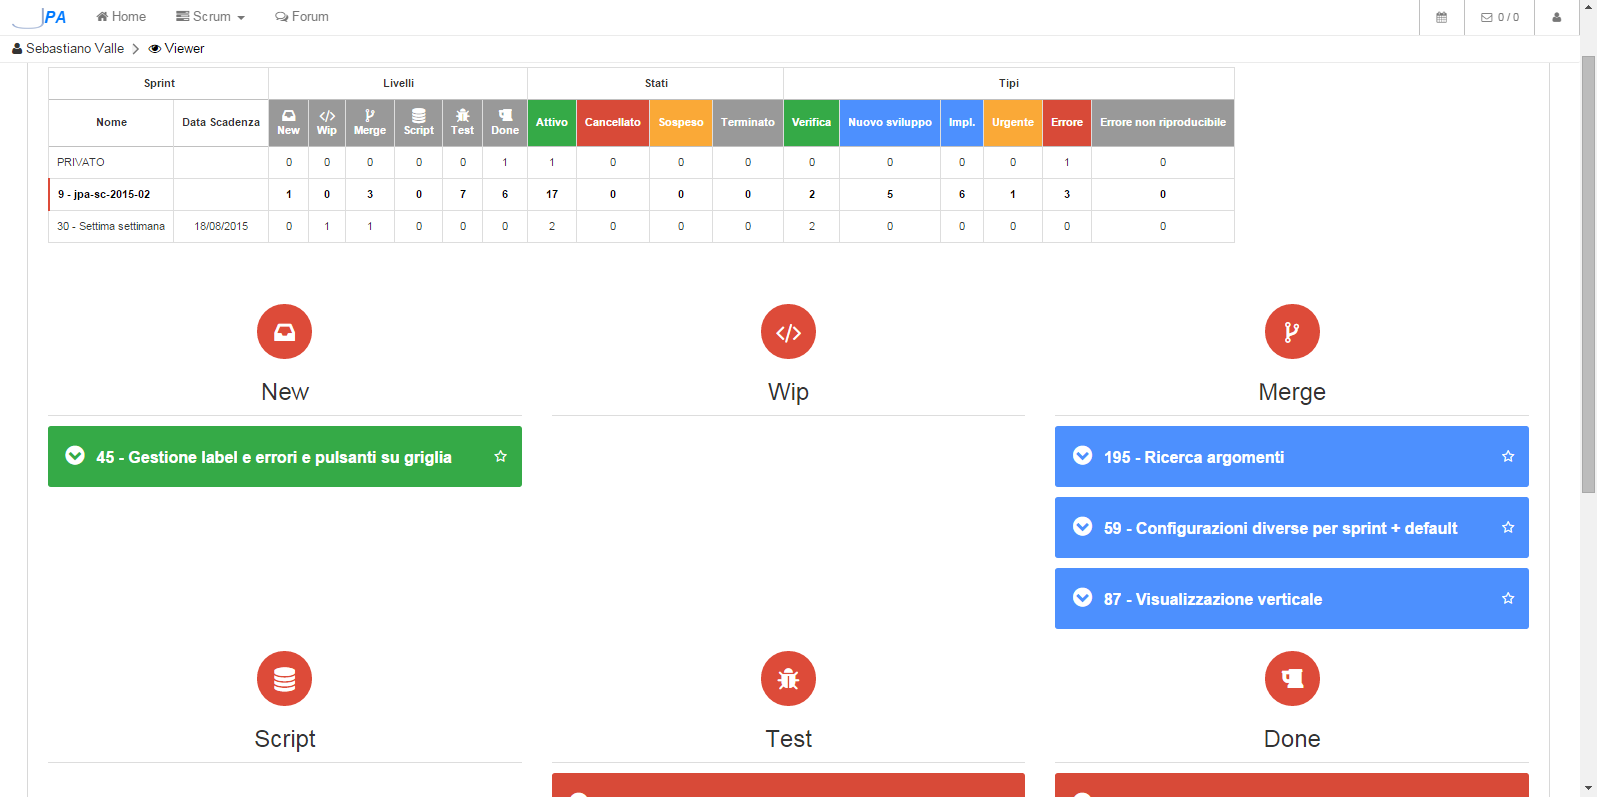
\includegraphics[width=\columnwidth]{immagini/jpa-sprint-viewer}%
\caption{Schermata di visualizzazione sprint in JPA}%
\label{fig:jpa-viewer}%
\end{figure}

Come è possibile vedere in figura \ref{fig:jpa-viewer}, i task possono essere
in diversi livelli a seconda del loro stato di avanzamento.

Questi livelli sono configurabili dall'amministratore di sistema e nel mio team
un task può passare per i seguenti stadi:

\begin{itemize}
	\item \textbf{New}, quando nessuno ha lavorato sul task e questo è ancora in
	analisi;
	\item \textbf{Wip}, quando uno o più membri del gruppo stanno lavorando sul
	task;
	\item \textbf{Merge}, in cui l'incremento dovuto al task viene integrato a
	JPA;
	\item \textbf{Script}, quando una modifica deve essere integrata tramite
	script (ad esempio l'inserimento di una riga in database);
	\item \textbf{Test}, in cui l'incremento prodotto dallo svolgimento del task
	viene controllato da un altro membro del gruppo;
	\item \textbf{Done}, in cui l'incremento prodotto da un task è definitivamente
	approvato ed integrato in JPA.
\end{itemize}

\begin{figure}%
\centering
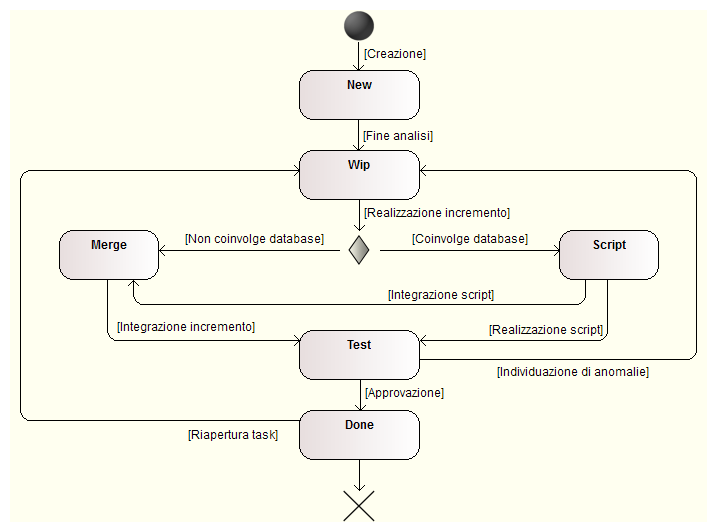
\includegraphics[width=.9\columnwidth]{immagini/task-life-cycle}%
\caption{Ciclo di vita di un task}%
\label{fig:task-lifecycle}%
\end{figure}

Oltre a questi livelli, è necessario indicare il \textbf{tipo} di un task, a
seconda della sua natura (Nuovo sviluppo, Implementazione, Urgente, Errore,
Errore non riproducibile).

Ogni task può essere preso in carico da uno o più operatori e vi si possono
aggiungere note o file in allegato.

\paragraph{Sprint privati} \mbox{}

JPA offre anche la possibilità di creare sprint privati, visibili solamente
all'utente che li ha creati, in cui vanno inseriti le attività di minore
importanza o dei task usati come promemoria.

\paragraph{Fine sprint} \mbox{}

Al termine di uno sprint, vi sono tre alternative possibili per ciascun task:

\begin{itemize}
	\item se un task è nello stato Done, è ritenuto concluso e JPA lo ignora;
	\item se un task è nello stato New, questo può essere assegnato ad un altro
	sprint o rimanere senza sprint;
	\item se un task è in uno dei rimanenti stati, \textbf{deve} essere
	riassegnato ad un altro sprint.
\end{itemize}

\subsection{JPADb}

JPADb è il database su cui JPA si appoggia. Tale base dati può essere gestita
da uno dei seguenti \gloss{rdbms}: MySQL, Firebird, DB2 400, MS SQL Server e DB2
UDB.

Le alterazioni alle tabelle o al loro contenuto avvengono tramite script Java,
utilizzando funzionalità del package \texttt{java.sql}.

Sebbene possa sembrare difficile applicare una modifica vista la diversa natura
dei vari \gloss{rdbms}, questo lavoro è notevolmente semplificato grazie ad
alcune \gloss{api} di JPA che consentono di eseguire i comandi di alterazione
delle tabelle e del loro contenuto in puro linguaggio SQL.

In questo modo lo sviluppatore può non essere a conoscenza dei dettagli di ogni
specifico sistema ed evitare di dover realizzare soluzioni complesse per delle
semplici operazioni come la creazione di una tabella ogni volta che si presenta
la necessità di compiere questo tipo di azione.

\paragraph{Norme e raccomandazioni per lo sviluppo} \mbox{} \\

Al momento del mio ingresso nel team, sono presenti le seguenti norme per la
creazione di tabelle in JPADb:

\begin{itemize}
	\item i nomi delle tabelle devono sempre riferirsi al plurale, in lingua
	inglese, agli elementi in essa contenuti. Eventuali deviazioni da tale regola
	devono essere discusse;
	\item i nomi delle tabelle devono sempre contenere il codice dell'area in cui
	vengono utilizzate come prefisso prima del nome degli elementi che questa
	contiene;
	\item una \gloss{chiaveprimaria} deve iniziare con \texttt{SEQ\_} e finire
	con il nome della tabella a cui è associata;
	\item una chiave esterna deve iniziare con \texttt{FK\_}, proseguire con il
	codice dell'area in cui viene utilizzata e un numero progressivo per
	distinguerla dalle altre della stessa area.
\end{itemize}

\subsection{Back-end}

Il lato server di JPA è realizzato con il linguaggio di programmazione Java.
Il \BKEND{} si decompone in \emph{WebServices} e \emph{WebShared}, per riuscire
rispettivamente ad accogliere le richieste dal client e delegarle al servizio
più adeguato.

Nella parte di \emph{WebServices} si trovano delle classi utilizzate per
accogliere le chiamate \gloss{rest} che provengono dal lato client. Per gestire
tali servizi, vengono utilizzate le \gloss{jaxrs} Jersey.

Affinchè i \emph{WebServices} siano leggeri e facilmente ritoccabili, tutta la
\emph{business logic} viene spostata nella parte di \emph{WebShared}, che
interagisce direttamente col database.

La parte di \emph{WebShared} non comunica direttamente con il client: per
questo motivo, i risultati delle operazioni sul database vengono consegnati
alla parte di \emph{WebServices} che si occupa di trasmetterli al \FREND{}.

JPA viene avviato e caricato sull'\gloss{applicationserver} Tomcat, il quale
viene a sua volta eseguito su una macchina virtuale le cui copie sono
utilizzate da tutti i membri del team.
La codifica, l'avvio dei server e il versionamento del codice avvengono
all'interno dell'\gloss{ide} Eclipse.

\paragraph{Versionamento} \mbox{} \\

La parte di \BKEND{} di JPA è versionata con il \gloss{vcs} SVN. Non vengono usati
particolari flussi di sviluppo, dal momento che tutte le modifiche vengono
applicate direttamente al ramo principale (\emph{trunk}) del
\gloss{repository}.

Ad ogni integrazione di una modifica al ramo principale, è obbligatorio
inserire un breve commento che descriva il cambiamento effettuato.

\paragraph{Norme e raccomandazioni per lo sviluppo} \mbox{} \\

Per quanto riguarda il lato server di JPA, gli sviluppatori sono tenuti a
seguire queste norme:

\begin{itemize}
	\item se una classe dei \emph{WebServices} fa parte di un'area (e.g.
	Scrum, avente codice \texttt{Sc}), il suo nome dovrà cominciare con il
	codice di questa;
	\item i metodi delle classi dei \emph{WebServices} devono essere statici;
	\item I metodi delle classi dei \emph{WebServices} devono avere dimensione
	ridotta (al massimo 20 righe), così da essere facilmente modificabili;
	\item gli URL che identificano i metodi della parte di \emph{WebServices}
	devono essere costituiti da insiemi di lettere lunghi al massimo tre
	lettere\footnote{Ad esempio il metodo \texttt{getList()} di una classe
	\texttt{ScSprint} nel package \texttt{plugins.sc} avrà un URL come
	\texttt{ws/pl/sc/s/l}, o simile}. Tale norma è legata a motivi di efficienza
	nell'eseguire chiamate \gloss{rest} al \BKEND{};
	\item usare sempre l'annotazione \texttt{@Override} quando una classe
	ridefinisce o concretizza un metodo della classe che estende o
	dell'interfaccia che implementa;
	\item usare sempre i metodi forniti dalle \gloss{api} di JPA per connettersi al
	database e chiudere la connessione a questo;
	\item il tempo di esecuzione di un metodo dei \emph{WebServices} deve essere
	sempre misurato;
	\item far corrispondere ad ogni classe \texttt{MyClass} nei
	\emph{WebServices} una classe \texttt{MyClassUtil} nella parte di
	\emph{WebShared} che soddisfi le richieste \gloss{rest} ricevute da
	\texttt{MyClass};
	\item ogni classe nella parte di model nei \emph{WebShared} deve avere il
	prefisso \texttt{Def};
	\item ogni metodo di una classe deve essere scritto rispettando le seguenti
	regole di stile:
	\begin{enumerate}
		\item le righe di istruzioni di importazione di package devono essere
		ordinate in ordine alfabetico;
		\item tra il nome di un metodo e le sue parentesi deve esserci uno spazio;
		\item le righe di codice vanno indentate;
		\item non bisogna usare il carattere di tabulazione per l'indentazione ma
		quattro spazi;
		\item è obbligatorio lasciare una riga vuota tra un metodo e l'altro;
		\item i nomi di classi devono essere scritti in \emph{UpperCamelCase};
		\item i nomi di metodi ed attributi devono essere scritti in
		\emph{lowerCamelCase};
		\item i nomi dei campi di un tipo enumerativo devono essere scritti in
		\emph{SNAKE\_CASE}, con tutti i caratteri in maiuscolo;
		\item ogni classe e ogni metodo devono avere il proprio nome aggiunto come
		commento nella linea in cui terminano.
	\end{enumerate}
\end{itemize}

Oltre alle regole sopra elencate, vi sono le seguenti raccomandazioni:

\begin{itemize}
	\item usare metodi statici anche nelle classi dei \emph{WebShared}, qualora
	possibile;
	\item commentare le parti di codice più complesse.
\end{itemize}

\paragraph{JPAUtil} \mbox{} \\

Nella parte di JPA dedicata alla modellazione di processi sono presenti
alcune \gloss{api} di utilità generica. Tali funzioni sono visibili a chi modella
un processo, la cui preparazione informatica può anche essere basilare.

Queste funzioni possono essere collegate ad un evento, ad esempio
l'approvazione di una richiesta di acquisto nella modellazione di un processo.

Per questo motivo, il team ha adottato le seguenti norme:

\begin{itemize}
	\item ogni funzione fornita da una \gloss{api} in JPAUtil deve verificare se
	la connessione al database è già aperta\footnote{Tale controllo alleggerisce
	notevolmente le responsabilità all'utilizzatore delle \gloss{api}}:
	\begin{itemize}
		\item Nel caso in cui lo fosse, utilizzare la connessione al database già
		esistente senza chiuderla al termine dell'operazione;
		\item Nel caso in cui non lo fosse, aprirne una propria e chiuderla al
		termine dell'operazione.
	\end{itemize}
	\item ad ogni metodo pubblico al quale viene richiesta un'operazione, ne deve
	corrispondere uno che esegue l'operazione richiesta;
	\item i metodi pubblici devono avere come \textbf{ultimo} parametro formale
	un oggetto di tipo \texttt{Connection}, mentre i metodi privati devono avere
	tale oggetto come \textbf{primo} parametro.
\end{itemize}

Siccome l'utilizzatore di queste \gloss{api} potrebbe disporre di una
preparazione informatica basilare, è raccomandato di preferire l'aggiunta di
parametri all'incapsulamento di questi in una classe.

Ciò è dovuto al fatto che molti possibili clienti dell'azienda potrebbero
non conoscere la programmazione ad oggetti e potrebbe risultare più facile per
questi elencare gli attributi di un oggetto piuttosto che far propri i
fondamenti di informatica necessari.

\subsection{Front-end}

Il lato client di JPA consiste in una \gloss{spa} realizzata con diverse
tecnologie:

\begin{itemize}
	\item HTML5 per la componente strutturale e semantica della pagina. Tale
	linguaggio è raccomandato dal \gloss{w3c} da ottobre 2014.
	\item TODC Bootstrap, un \gloss{framework} open source derivato da Bootstrap
	di Twitter. Sviluppato da una comunità di designer web, usa CSS3 e fornisce
	uno stile alle pagine simile a quello di Google;
	\item AngularJS, un \gloss{framework} che guida lo sviluppo di \gloss{spa}
	con elementi architetturali che si ispirano al pattern MVC.
\end{itemize}

Il browser su cui viene provata JPA è Chromium, mentre il codice del \FREND{}
viene scritto utilizzando Sublime Text 2.

L'applicazione \FREND{} di JPA al momento ha come lingue disponibili l'italiano
e l'inglese. Tuttavia l'aggiunta di nuovi dizionari è semplice poichè i testi
delle viste HTML sono gestiti in modo automatico da JPA tramite un dizionario.

\paragraph{Versionamento} \mbox{} \\

A differenza del \BKEND{}, il lato client non dispone di un \gloss{vcs}.

Per questo motivo, quando gli incrementi per il \FREND{} vengono sviluppati,
vanno allegati in JPA passando al livello Merge in modo tale che possano essere
integrati in JPA da Alex Beggiato, una volta testati.

Non essendovi un \gloss{repository} di accesso comune, i file utilizzati vengono
distribuiti ad intervalli non definiti, solitamente quando un membro deve
effettuare una modifica su una parte su cui un altro componente del team ha
cambiato parte del codice.

Nel caso in cui due persone avessero modificato lo stesso file nel \FREND{}, si
raccomanda di usare \textbf{Meld} per unire i due file, anche se ciascun
componente del team è libero di utilizzare lo strumento che preferisce.

\paragraph{Norme e raccomandazioni per lo sviluppo} \mbox{} \\

Al momento del mio ingresso nel team, sono presenti le seguenti norme per lo
sviluppo del lato client di JPA:

\begin{itemize}
\item ogni variabile locale ad una funzione deve essere preceduta dalla parola
chiave \texttt{var} nella sua dichiarazione, poichè vengono utilizzate diverse
variabili e funzioni globali;
\item le parti di testo visualizzate in JPA sono proprietà dell'oggetto
\texttt{\$scope.\_label} e devono essere lette con la funzione
\texttt{\_getLabelFor()}, la quale a sua volta utilizza dei file di
configurazione contenenti delle parole o delle frasi in diverse lingue;
\item ogni statement deve essere concluso con un punto e virgola;
\item assegnare un codice univoco ad ogni errore. L'ultimo codice di errore
utilizzato per una certa area è riportato nell'area Forum di JPA;
\item in ogni chiamata che esegue una chiamata \gloss{rest} verso il \BKEND{},
impedire l'uso della pagina all'utente  mostrando una schermata di attesa fino
al termine dell'operazione;
\item anteporre \texttt{data-} ai nomi delle direttive di AngularJS nei tag
HTML;
\item i nomi delle funzioni devono cominciare con ``\texttt{on}'' se invocate
direttamente da un elemento della vista HTML.
\end{itemize}

\section{Propensione all'innovazione}

Sanmarco Informatica compie molti sforzi per rimanere aggiornata ed essere
innovativa e competitiva sul mercato.

\subsection{Investimento nella ricerca} \mbox{}

Durante il periodo del mio stage ho lavorato al centro aziendale di Ricerca,
Sviluppo e Formazione. In questa sede, oltre al miglioramento e alla
manutenzione di funzionalità già presenti nei software in commercio, vengono
svolte anche attività di ricerca e prototipazione (come è successo nel caso
del mio stage).

L'azienda procede in modo deciso in questa direzione: l'investimento medio del
proprio fatturato in ricerca da quando l'azienda è nata corrisponde al 17\%,
mentre negli ultimi due anni (2013 e 2014) è arrivato al 20\% per ciascun anno.

Questa scelta ha portato i suoi benefici, aiutando l'azienda ad avere dei
risultati economici nettamente in contrasto con l'andamento del resto
dell'economia nazionale: il bilancio del 2014 si è chiuso con un incremento del
34\%, mentre la crescita prospettata per la fine del corrente anno è del 40\%.

I guadagni ottenuti hanno consentito all'azienda di investire anche assumendo
13 nuovi dipendenti, di cui 5 ricercatori.

\subsection{OpenPOWER Foundation} \mbox{}

Sanmarco Informatica è la prima ed unica azienda italiana che è entrata a far
parte (ad inizio 2015) della prestigiosa fondazione \textbf{OpenPOWER
Foundation}.

Tale consorzio, creato da Google, IBM, Mellanox Technologies, Tyan, Samsung e
Nvidia è una comunità i cui partner collaborano per ricavare un'opportunità di
crescita e riuscire ad adeguarsi all'evoluzione dei bisogni dei clienti.
Questo obiettivo viene raggiunto da OpenPOWER Foundation condividendo
competenze e investimento nella ricerca da parte di aziende ed università.

Entrando in OpenPOWER Foundation, Sanmarco Informatica ha deciso di offrire il
suo contributo sviluppando PowerJ (una nuova versione di Jgalileo), un
\gloss{erp} basato su tecnologie open source, in grado di offrire risparmi in
costi di licenza, preferendo tecnologie opensource ad alternative proprietarie.

Con questo prodotto il cliente può disporre del cosiddetto sistema ``Cloud On
Site'': PowerJ semplifica l'uso di una piattaforma Cloud proteggendo i dati ed
integrando le applicazioni sulla piattaforma Cloud con quelle in locale.

\begin{figure}%
\centering
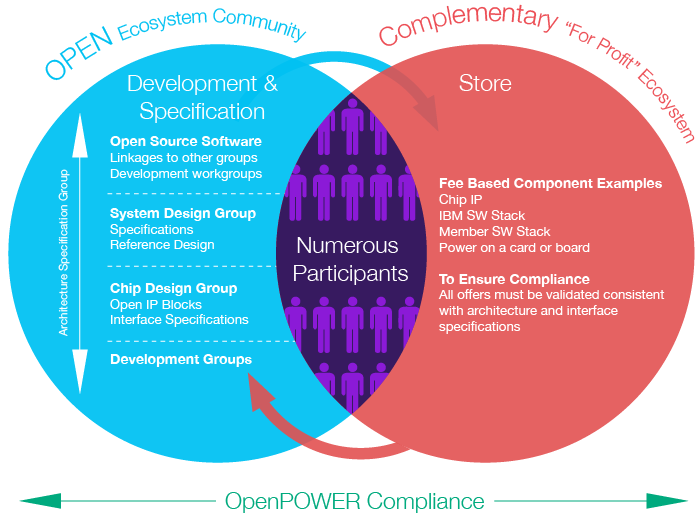
\includegraphics[width=.7\columnwidth]{immagini/open-power-foundation}%
\caption{Come OpenPOWER Foundation fornisce supporto alle aziende}%
\label{fig:open-power-foundation}%
\end{figure}

\subsection{4words} \mbox{}

La propensione all'innovazione di Sanmarco Informatica è confermata anche
dall'esistenza di progetti come \textbf{4words}, web agency che prende il suo
nome da quattro valori a cui dichiara di ispirarsi: efficacia, funzionalità,
flessibilità e innovazione.

Questo team si occupa principalmente di realizzazione di siti Web e promozione
online per aziende. Grazie ai suoi servizi, le aziende riescono a guadagnare
visibilità rispetto al consumatore, migliorando l'efficacia del proprio sito in
termini di indicizzazione da parte di Google (\textbf{SEO}) e promuovendo il
proprio marchio nei social network.

Al momento il progetto si sta muovendo verso il futuro cercando di anticipare
l'evoluzione dei motori di ricerca. Per far ciò, uno degli obiettivi attuali
del progetto è costruire delle mappe linguistiche che possano essere integrate
nei siti favorendo l'indicizzazione semantica e permettendo di farsi trovare
più facilmente dall'utente.

\subsection{Prodotti} \mbox{}

Sanmarco Informatica si propone in modo innovativo al cliente anche per quanto
riguarda alcune delle tecnologie che utilizza per sviluppare i propri prodotti.

La decisione dell'azienda è ambiziosa e al contempo coraggiosa: i prodotti che
offre gestiscono la pianificazione delle risorse di aziende, un campo dove
errori o comportamenti inattesi dovuti a tecnologie poco stabili possono
costare molto.

Sanmarco Informatica agisce sviluppando soluzioni che siano robuste e stabili
sul lato server dei propri software, affidandosi a un colosso dell'informatica
come IBM e a tecnologie stabili ed affermate come Java e SQL.

Allo stesso tempo, si mantiene moderna sperimentando vari modi per far
interagire gli utenti con le proprie applicazioni: le tecnologie utilizzate (ad
esempio AngularJS) spesso sono molto giovani e sono soggette al rischio di
mutazioni drastiche nel giro di brevi periodi.

L'azienda non trascura il mondo \emph{mobile}: le applicazioni Web sono
\gloss{responsive} e vi sono progetti che si occupano esclusivamente dello
sviluppo di applicazioni per smartphone e tablet.

\subsection{Personale} \mbox{}

Quanto visto per le tecnologie utilizzate per i propri prodotti si riflette sul
personale all'interno dell'azienda, che combina saggiamente esperienza con le
menti fresche di giovani, provenienti sia da scuole superiori che da
università.

Ogni anno Sanmarco Informatica offre infatti molteplici opportunità di attività
di stage, nelle quali i giovani possono dare il loro contributo alla software
house potendo lavorare su tecnologie accattivanti ed al contempo guadagnado
utile esperienza.

\subsection{Scrum} \mbox{}

Un ulteriore aspetto in cui si può notare la propensione all'innovazione di
Sanmarco Informatica sta nel fatto di aver adottato la metodologia Scrum.

Non era scontato che un'azienda operante da circa venticinque anni che produce
software gestionale decidesse di cambiare il modello con cui i processi e le
persone sono organizzate per lo sviluppo dei propri prodotti.

Questa scelta coraggiosa ha rinfrescato l'azienda, snellendo i processi e ha
permesso di riuscire meglio nel rispettare scadenze e a far fronte a
tempistiche pressanti.
